\section{Algorytm A*}
\subsection{Geneza powstania}
Algorytm A* powstał w ramach projektu Shakey, zapoczątkowanego w 1966 roku przez Charles Rosen'a.
Celem projektu było zbudowanie robota, który potrafiłby planować własne działania. 
Zbudowany robot wyróżniał się na tle innych tym że intergował kilka różnych modeli sztuczenj 
inteligencji pracujących jako jeden system.

Robot był zbudowany z:
- kamery telewizyjnej i dalmierza optycznego - system wizyjny do obserwacji środowiska
- łącze radiowe - służącego do komunikacji z bazą, odbierania i wysyłania komend
- detektor uderzeń - pozwalający na zatrzymanie robota w przypadku kolizji

Komunikacja odbywała się poprzez wysyłane radiowo tekstowe polecenia mające określoną strukturę np.:
GOTO D4 - co oznaczało automatyczne przemieszczenie się robota do wskazanej pozycji
\begin{figure}[H]
	\centering
	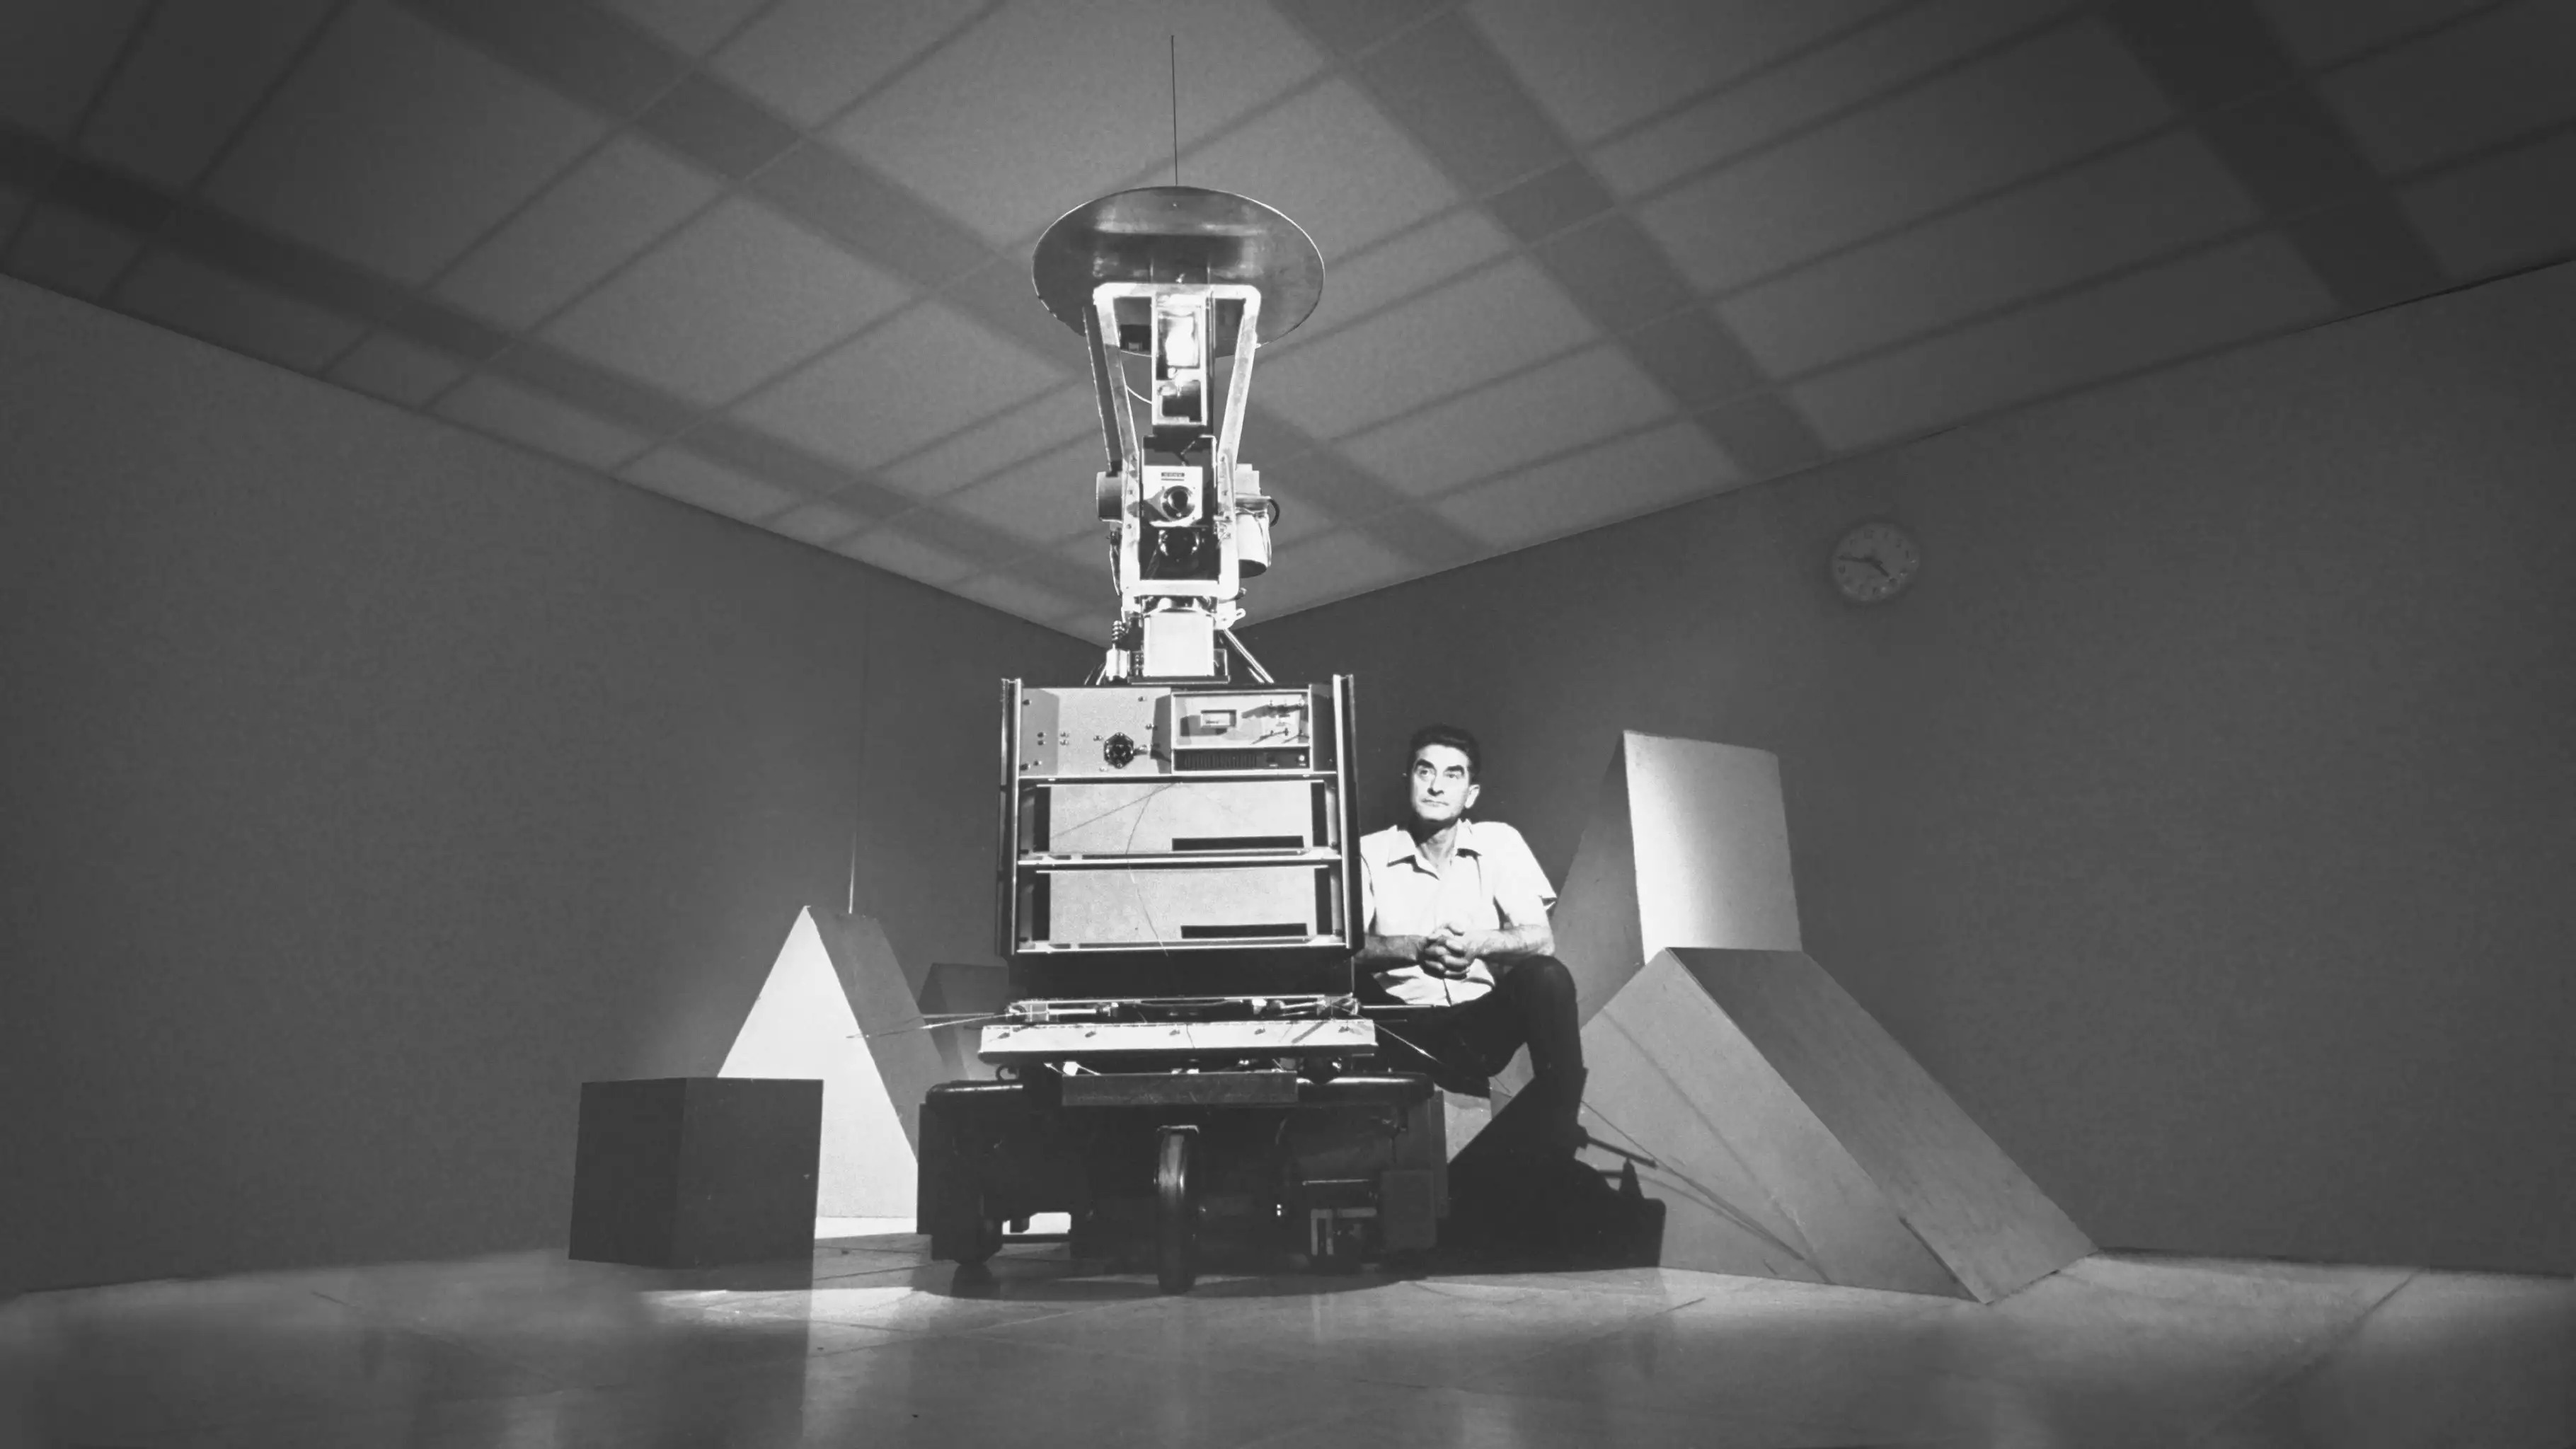
\includegraphics[width=14cm]{pages/algorytm/zdjecia/shakey2.jpg}
	\caption{Robot Shakey i Charles Rosen, inicjator projektu \cite{robotShakey}}
	\label{fig:Rys}
\end{figure}

\subsection{Opis działania algorytmu}

A* to heurestyczny algorytm wyznaczający najkrótszą możliwą ścieżkę w grafie. 
Jest to algorytm zupełny i optymalny, a więc zawsze zostanie wyznaczone optymalne 
rozwiązanie. Ze względu na przeszukiwanie oparte na grafie algorytm działa najlepiej na strukturze drzewiastej.
Zadaniem algorytmu jest minimalizacja funkcji:
\begin{equation}
	f(x)=h(x) + g(x)
	\label{Eq:funkcjaKosztuAStar}
\end{equation}
gdzie: $f(x)$ - minimalizowana funkcja, $g(x)$ - to rzeczywisty koszt dojścia do punktu x.

Funkcja $h(x)$ to funkcja heurestyczna, oszacowuje ona koszt dotarcia od punktu x do wierzchołka docelowego

Zalety:
\begin{itemize}
	\item jest kompletny i optymalny
	\item może przeszukiwać skomplikowane mapy
	\item jest najwydajniejszym takim algorytmem
\end{itemize}
Wady:
\begin{itemize}
	\item jego wydajność w znacznej mierze zależy od funkcji heurestycznej
	\item Każda akcja ma stały koszt wykonania
	\item nie nadaje się do często zmieniającego się otoczenia robota, wymaga ponownego przeliczenia
\end{itemize}


\textbf{Przykładowe funkcje heurestyczne:}
\begin{itemize}
	\item Funkcja euklidesowa
	      \begin{equation}
	      	h(x)= 10 * \sqrt[2]{(x_1 - x_2)^2 + (y_1 - y_2)^2}
	      	\label{Eq:heuresticEucalides}
	      \end{equation}
	\item Geometria Manhattanu (innaczej metryka miejska)
	      \begin{equation}
	      	h(x)= |x_2 - x_1| + |y_2 - y_1|
	      	\label{Eq:heuresticManhattanu}
	      \end{equation}
\end{itemize}
Gdzie: $x_1$ i $y_1$ to współrzędne wyznaczanego punktu, $x_2$ i $y_2$ to koordynaty celu


%TODO: cos o innych algorytmach np. skanowaine otoczenia lidarem

